\documentclass{standalone}
\usepackage{tikz}
\usetikzlibrary{patterns, positioning}
\usepackage[sfdefault]{ClearSans} %% option 'sfdefault' activates Clear Sans as the default text font
\usepackage[T1]{fontenc}

\begin{document}
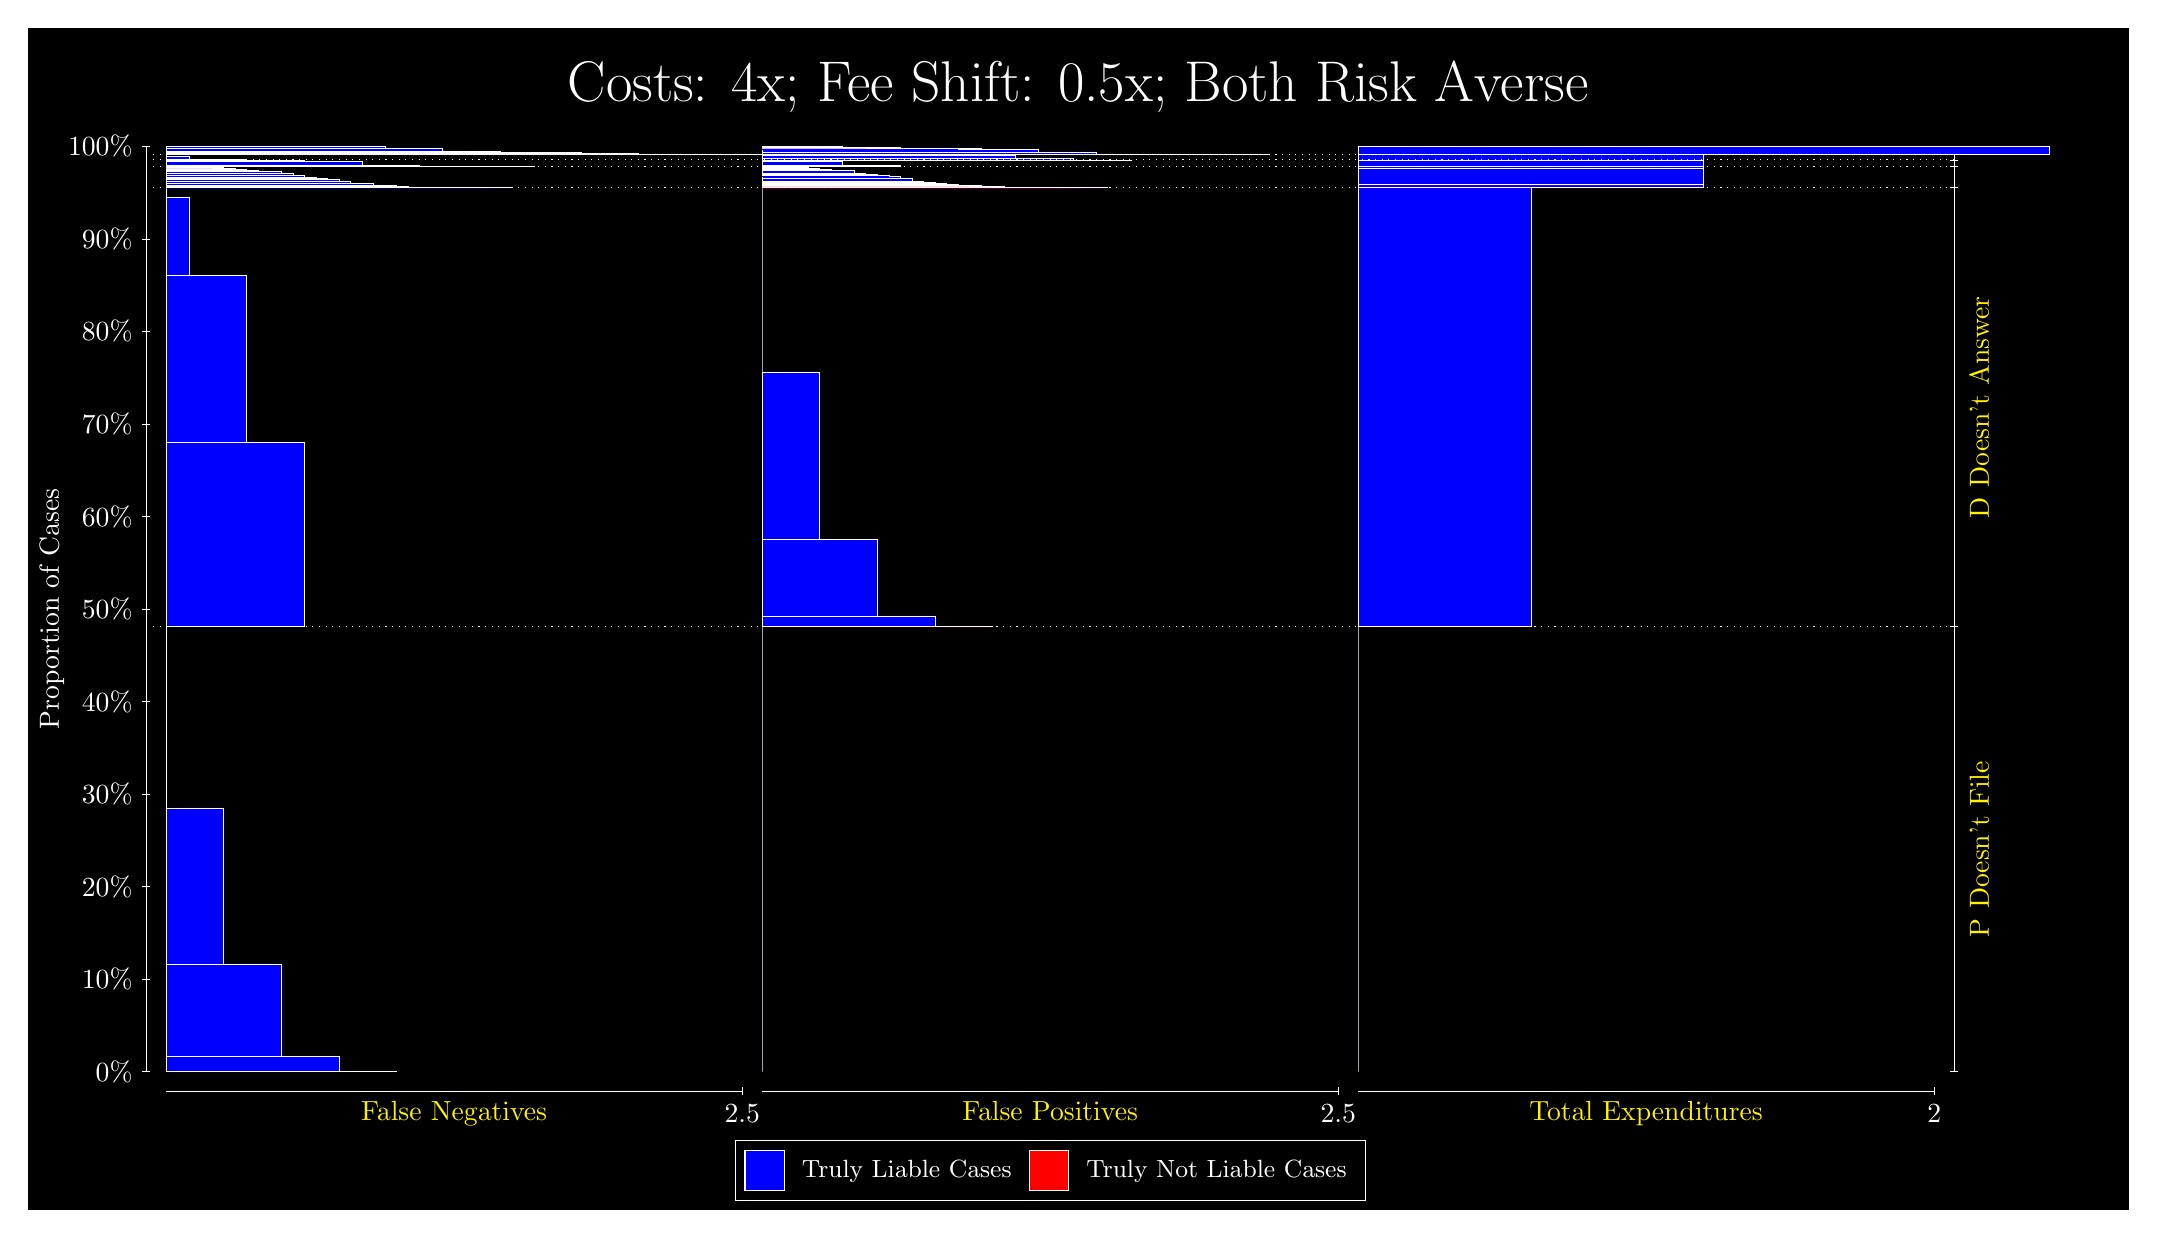
\begin{tikzpicture}
\draw[fill=black] (0,0) rectangle (26.667,15);
\draw[text=white] (0,13.5) rectangle (26.667,15) node[midway] {\huge Costs: 4x; Fee Shift: 0.5x; Both Risk Averse};
\draw[white, very thin] (1.5,1.75) -- (1.5,13.5);
\node[rotate=90, text=white, anchor=center] at (0.3, 7.625) {Proportion of Cases};
\draw[white, very thin] (1.45,1.75) -- (1.55,1.75);
\node[text=white, anchor=east] at (1.45, 1.75) {0\%};
\draw[white, very thin] (1.45,2.925) -- (1.55,2.925);
\node[text=white, anchor=east] at (1.45, 2.925) {10\%};
\draw[white, very thin] (1.45,4.1) -- (1.55,4.1);
\node[text=white, anchor=east] at (1.45, 4.1) {20\%};
\draw[white, very thin] (1.45,5.275) -- (1.55,5.275);
\node[text=white, anchor=east] at (1.45, 5.275) {30\%};
\draw[white, very thin] (1.45,6.45) -- (1.55,6.45);
\node[text=white, anchor=east] at (1.45, 6.45) {40\%};
\draw[white, very thin] (1.45,7.625) -- (1.55,7.625);
\node[text=white, anchor=east] at (1.45, 7.625) {50\%};
\draw[white, very thin] (1.45,8.8) -- (1.55,8.8);
\node[text=white, anchor=east] at (1.45, 8.8) {60\%};
\draw[white, very thin] (1.45,9.975) -- (1.55,9.975);
\node[text=white, anchor=east] at (1.45, 9.975) {70\%};
\draw[white, very thin] (1.45,11.15) -- (1.55,11.15);
\node[text=white, anchor=east] at (1.45, 11.15) {80\%};
\draw[white, very thin] (1.45,12.325) -- (1.55,12.325);
\node[text=white, anchor=east] at (1.45, 12.325) {90\%};
\draw[white, very thin] (1.45,13.5) -- (1.55,13.5);
\node[text=white, anchor=east] at (1.45, 13.5) {100\%};

\draw[white, very thin] (24.457,1.75) -- (24.457,13.5);
\draw[white, very thin] (24.407,1.75) -- (24.507,1.75);
\node[anchor=west] at (24.407, 1.75) {};
\draw[white, very thin] (24.407,7.399) -- (24.507,7.399);
\node[anchor=west] at (24.407, 7.399) {};
\draw[white, very thin] (24.407,12.977) -- (24.507,12.977);
\node[anchor=west] at (24.407, 12.977) {};
\draw[white, very thin] (24.407,13.245) -- (24.507,13.245);
\node[anchor=west] at (24.407, 13.245) {};
\draw[white, very thin] (24.407,13.328) -- (24.507,13.328);
\node[anchor=west] at (24.407, 13.328) {};
\draw[white, very thin] (24.407,13.398) -- (24.507,13.398);
\node[anchor=west] at (24.407, 13.398) {};
\draw[white, very thin] (24.407,13.5) -- (24.507,13.5);
\node[anchor=west] at (24.407, 13.5) {};

\draw[white, very thin, fill=blue] (1.75,1.75) rectangle (4.6775,1.7519);
\draw[white, very thin, fill=blue] (1.75,1.7519) rectangle (3.9457,1.9459);
\draw[white, very thin, fill=blue] (1.75,1.9459) rectangle (3.2138,3.1068);
\draw[white, very thin, fill=blue] (1.75,3.1068) rectangle (2.4819,5.0989);
\draw[white, very thin, fill=red] (1.75,5.0989) rectangle (1.75,5.0989);
\draw[white, very thin, fill=blue] (1.75,5.0989) rectangle (1.75,7.399);
\draw[white, very thin, fill=blue] (1.75,7.399) rectangle (3.5065,9.7466);
\draw[white, very thin, fill=blue] (1.75,9.7466) rectangle (2.7746,11.868);
\draw[white, very thin, fill=blue] (1.75,11.868) rectangle (2.0428,12.848);
\draw[white, very thin, fill=red] (1.75,12.848) rectangle (1.75,12.848);
\draw[white, very thin, fill=blue] (1.75,12.848) rectangle (1.75,12.977);
\draw[white, very thin, fill=blue] (1.75,12.977) rectangle (6.1413,12.977);
\draw[white, very thin, fill=blue] (1.75,12.977) rectangle (5.8486,12.977);
\draw[white, very thin, fill=blue] (1.75,12.977) rectangle (5.5558,12.977);
\draw[white, very thin, fill=blue] (1.75,12.977) rectangle (5.4094,12.98);
\draw[white, very thin, fill=blue] (1.75,12.98) rectangle (5.2631,12.98);
\draw[white, very thin, fill=blue] (1.75,12.98) rectangle (5.1167,12.985);
\draw[white, very thin, fill=blue] (1.75,12.985) rectangle (4.9703,12.985);
\draw[white, very thin, fill=blue] (1.75,12.985) rectangle (4.8239,12.989);
\draw[white, very thin, fill=blue] (1.75,12.989) rectangle (4.6775,13.005);
\draw[white, very thin, fill=blue] (1.75,13.005) rectangle (4.5312,13.008);
\draw[white, very thin, fill=blue] (1.75,13.008) rectangle (4.3848,13.008);
\draw[white, very thin, fill=blue] (1.75,13.008) rectangle (4.3848,13.027);
\draw[white, very thin, fill=blue] (1.75,13.027) rectangle (4.2384,13.031);
\draw[white, very thin, fill=blue] (1.75,13.031) rectangle (4.092,13.062);
\draw[white, very thin, fill=blue] (1.75,13.062) rectangle (4.092,13.062);
\draw[white, very thin, fill=blue] (1.75,13.062) rectangle (3.9457,13.079);
\draw[white, very thin, fill=blue] (1.75,13.079) rectangle (3.7993,13.093);
\draw[white, very thin, fill=blue] (1.75,13.093) rectangle (3.6529,13.095);
\draw[white, very thin, fill=blue] (1.75,13.095) rectangle (3.6529,13.107);
\draw[white, very thin, fill=blue] (1.75,13.107) rectangle (3.5065,13.126);
\draw[white, very thin, fill=blue] (1.75,13.126) rectangle (3.3602,13.162);
\draw[white, very thin, fill=blue] (1.75,13.162) rectangle (3.3602,13.163);
\draw[white, very thin, fill=blue] (1.75,13.163) rectangle (3.2138,13.179);
\draw[white, very thin, fill=blue] (1.75,13.179) rectangle (3.0674,13.182);
\draw[white, very thin, fill=blue] (1.75,13.182) rectangle (3.0674,13.189);
\draw[white, very thin, fill=blue] (1.75,13.189) rectangle (2.921,13.196);
\draw[white, very thin, fill=blue] (1.75,13.196) rectangle (2.921,13.199);
\draw[white, very thin, fill=blue] (1.75,13.199) rectangle (2.7746,13.212);
\draw[white, very thin, fill=blue] (1.75,13.212) rectangle (2.6283,13.219);
\draw[white, very thin, fill=blue] (1.75,13.219) rectangle (2.6283,13.221);
\draw[white, very thin, fill=blue] (1.75,13.221) rectangle (2.4819,13.231);
\draw[white, very thin, fill=blue] (1.75,13.231) rectangle (2.3355,13.231);
\draw[white, very thin, fill=blue] (1.75,13.231) rectangle (2.3355,13.234);
\draw[white, very thin, fill=blue] (1.75,13.234) rectangle (2.1891,13.239);
\draw[white, very thin, fill=blue] (1.75,13.239) rectangle (2.0428,13.239);
\draw[white, very thin, fill=blue] (1.75,13.239) rectangle (1.8964,13.242);
\draw[white, very thin, fill=red] (1.75,13.242) rectangle (1.75,13.242);
\draw[white, very thin, fill=blue] (1.75,13.242) rectangle (1.75,13.245);
\draw[white, very thin, fill=blue] (1.75,13.245) rectangle (6.4341,13.245);
\draw[white, very thin, fill=blue] (1.75,13.245) rectangle (5.7022,13.246);
\draw[white, very thin, fill=blue] (1.75,13.246) rectangle (4.9703,13.264);
\draw[white, very thin, fill=blue] (1.75,13.264) rectangle (4.2384,13.311);
\draw[white, very thin, fill=blue] (1.75,13.311) rectangle (3.5065,13.328);
\draw[white, very thin, fill=red] (1.75,13.328) rectangle (1.75,13.328);
\draw[white, very thin, fill=blue] (1.75,13.328) rectangle (3.5065,13.328);
\draw[white, very thin, fill=blue] (1.75,13.328) rectangle (2.7746,13.336);
\draw[white, very thin, fill=blue] (1.75,13.336) rectangle (2.0428,13.371);
\draw[white, very thin, fill=red] (1.75,13.371) rectangle (1.75,13.371);
\draw[white, very thin, fill=blue] (1.75,13.371) rectangle (1.75,13.398);
\draw[white, very thin, fill=blue] (1.75,13.398) rectangle (9.9471,13.398);
\draw[white, very thin, fill=blue] (1.75,13.398) rectangle (9.2152,13.398);
\draw[white, very thin, fill=blue] (1.75,13.398) rectangle (8.4834,13.399);
\draw[white, very thin, fill=blue] (1.75,13.399) rectangle (7.7515,13.413);
\draw[white, very thin, fill=blue] (1.75,13.413) rectangle (7.4587,13.413);
\draw[white, very thin, fill=blue] (1.75,13.413) rectangle (7.0196,13.427);
\draw[white, very thin, fill=blue] (1.75,13.427) rectangle (6.7268,13.427);
\draw[white, very thin, fill=blue] (1.75,13.427) rectangle (6.2877,13.428);
\draw[white, very thin, fill=blue] (1.75,13.428) rectangle (5.9949,13.435);
\draw[white, very thin, fill=blue] (1.75,13.435) rectangle (5.5558,13.435);
\draw[white, very thin, fill=blue] (1.75,13.435) rectangle (5.2631,13.474);
\draw[white, very thin, fill=blue] (1.75,13.474) rectangle (4.5312,13.498);
\draw[white, very thin, fill=blue] (1.75,13.498) rectangle (3.7993,13.5);
\draw[white, very thin, fill=blue] (1.75,13.5) rectangle (3.0674,13.5);
\draw[white, very thin, fill=blue] (1.75,13.5) rectangle (2.3355,13.5);
\draw[white, very thin, fill=red] (1.75,13.5) rectangle (1.75,13.5);
\draw[white, very thin, fill=red] (9.3189,1.75) rectangle (9.3189,1.75);
\draw[white, very thin, fill=blue] (9.3189,1.75) rectangle (9.3189,7.399);
\draw[white, very thin, fill=red] (9.3189,7.399) rectangle (12.246,7.399);
\draw[white, very thin, fill=blue] (9.3189,7.399) rectangle (12.246,7.4019);
\draw[white, very thin, fill=blue] (9.3189,7.4019) rectangle (11.515,7.5278);
\draw[white, very thin, fill=blue] (9.3189,7.5278) rectangle (10.783,8.5079);
\draw[white, very thin, fill=blue] (9.3189,8.5079) rectangle (10.051,10.63);
\draw[white, very thin, fill=blue] (9.3189,10.63) rectangle (9.3189,12.977);
\draw[white, very thin, fill=red] (9.3189,12.977) rectangle (13.71,12.977);
\draw[white, very thin, fill=blue] (9.3189,12.977) rectangle (13.71,12.977);
\draw[white, very thin, fill=red] (9.3189,12.977) rectangle (13.417,12.977);
\draw[white, very thin, fill=blue] (9.3189,12.977) rectangle (13.417,12.977);
\draw[white, very thin, fill=red] (9.3189,12.977) rectangle (13.125,12.977);
\draw[white, very thin, fill=blue] (9.3189,12.977) rectangle (13.125,12.978);
\draw[white, very thin, fill=blue] (9.3189,12.978) rectangle (12.978,12.98);
\draw[white, very thin, fill=red] (9.3189,12.98) rectangle (12.832,12.98);
\draw[white, very thin, fill=blue] (9.3189,12.98) rectangle (12.832,12.98);
\draw[white, very thin, fill=blue] (9.3189,12.98) rectangle (12.686,12.983);
\draw[white, very thin, fill=red] (9.3189,12.983) rectangle (12.539,12.983);
\draw[white, very thin, fill=blue] (9.3189,12.983) rectangle (12.539,12.983);
\draw[white, very thin, fill=blue] (9.3189,12.983) rectangle (12.393,12.988);
\draw[white, very thin, fill=red] (9.3189,12.988) rectangle (12.246,12.988);
\draw[white, very thin, fill=blue] (9.3189,12.988) rectangle (12.246,12.991);
\draw[white, very thin, fill=blue] (9.3189,12.991) rectangle (12.1,13.001);
\draw[white, very thin, fill=red] (9.3189,13.001) rectangle (11.954,13.001);
\draw[white, very thin, fill=blue] (9.3189,13.001) rectangle (11.954,13.01);
\draw[white, very thin, fill=blue] (9.3189,13.01) rectangle (11.807,13.023);
\draw[white, very thin, fill=red] (9.3189,13.023) rectangle (11.661,13.023);
\draw[white, very thin, fill=blue] (9.3189,13.023) rectangle (11.661,13.026);
\draw[white, very thin, fill=blue] (9.3189,13.026) rectangle (11.661,13.033);
\draw[white, very thin, fill=blue] (9.3189,13.033) rectangle (11.515,13.043);
\draw[white, very thin, fill=red] (9.3189,13.043) rectangle (11.368,13.043);
\draw[white, very thin, fill=blue] (9.3189,13.043) rectangle (11.368,13.06);
\draw[white, very thin, fill=blue] (9.3189,13.06) rectangle (11.222,13.096);
\draw[white, very thin, fill=blue] (9.3189,13.096) rectangle (11.075,13.115);
\draw[white, very thin, fill=blue] (9.3189,13.115) rectangle (10.929,13.127);
\draw[white, very thin, fill=blue] (9.3189,13.127) rectangle (10.929,13.129);
\draw[white, very thin, fill=blue] (9.3189,13.129) rectangle (10.783,13.143);
\draw[white, very thin, fill=blue] (9.3189,13.143) rectangle (10.636,13.16);
\draw[white, very thin, fill=blue] (9.3189,13.16) rectangle (10.49,13.191);
\draw[white, very thin, fill=blue] (9.3189,13.191) rectangle (10.344,13.195);
\draw[white, very thin, fill=blue] (9.3189,13.195) rectangle (10.197,13.214);
\draw[white, very thin, fill=blue] (9.3189,13.214) rectangle (10.197,13.214);
\draw[white, very thin, fill=blue] (9.3189,13.214) rectangle (10.051,13.217);
\draw[white, very thin, fill=blue] (9.3189,13.217) rectangle (9.9044,13.233);
\draw[white, very thin, fill=blue] (9.3189,13.233) rectangle (9.758,13.237);
\draw[white, very thin, fill=blue] (9.3189,13.237) rectangle (9.6116,13.237);
\draw[white, very thin, fill=blue] (9.3189,13.237) rectangle (9.4652,13.242);
\draw[white, very thin, fill=blue] (9.3189,13.242) rectangle (9.3189,13.245);
\draw[white, very thin, fill=red] (9.3189,13.245) rectangle (11.075,13.245);
\draw[white, very thin, fill=blue] (9.3189,13.245) rectangle (11.075,13.262);
\draw[white, very thin, fill=blue] (9.3189,13.262) rectangle (10.344,13.309);
\draw[white, very thin, fill=blue] (9.3189,13.309) rectangle (9.6116,13.327);
\draw[white, very thin, fill=blue] (9.3189,13.327) rectangle (9.3189,13.328);
\draw[white, very thin, fill=red] (9.3189,13.328) rectangle (14.003,13.328);
\draw[white, very thin, fill=blue] (9.3189,13.328) rectangle (14.003,13.329);
\draw[white, very thin, fill=blue] (9.3189,13.329) rectangle (13.271,13.354);
\draw[white, very thin, fill=blue] (9.3189,13.354) rectangle (12.539,13.389);
\draw[white, very thin, fill=blue] (9.3189,13.389) rectangle (11.807,13.398);
\draw[white, very thin, fill=blue] (9.3189,13.398) rectangle (11.075,13.398);
\draw[white, very thin, fill=red] (9.3189,13.398) rectangle (15.759,13.398);
\draw[white, very thin, fill=blue] (9.3189,13.398) rectangle (15.759,13.398);
\draw[white, very thin, fill=blue] (9.3189,13.398) rectangle (15.028,13.398);
\draw[white, very thin, fill=red] (9.3189,13.398) rectangle (15.028,13.398);
\draw[white, very thin, fill=blue] (9.3189,13.398) rectangle (15.028,13.398);
\draw[white, very thin, fill=blue] (9.3189,13.398) rectangle (14.296,13.399);
\draw[white, very thin, fill=red] (9.3189,13.399) rectangle (14.296,13.399);
\draw[white, very thin, fill=blue] (9.3189,13.399) rectangle (14.296,13.4);
\draw[white, very thin, fill=blue] (9.3189,13.4) rectangle (13.564,13.401);
\draw[white, very thin, fill=red] (9.3189,13.401) rectangle (13.564,13.401);
\draw[white, very thin, fill=blue] (9.3189,13.401) rectangle (13.564,13.423);
\draw[white, very thin, fill=blue] (9.3189,13.423) rectangle (12.832,13.423);
\draw[white, very thin, fill=blue] (9.3189,13.423) rectangle (12.832,13.463);
\draw[white, very thin, fill=red] (9.3189,13.463) rectangle (12.539,13.463);
\draw[white, very thin, fill=blue] (9.3189,13.463) rectangle (12.539,13.463);
\draw[white, very thin, fill=blue] (9.3189,13.463) rectangle (12.1,13.469);
\draw[white, very thin, fill=blue] (9.3189,13.469) rectangle (11.807,13.47);
\draw[white, very thin, fill=red] (9.3189,13.47) rectangle (11.807,13.47);
\draw[white, very thin, fill=blue] (9.3189,13.47) rectangle (11.807,13.471);
\draw[white, very thin, fill=blue] (9.3189,13.471) rectangle (11.368,13.471);
\draw[white, very thin, fill=blue] (9.3189,13.471) rectangle (11.075,13.472);
\draw[white, very thin, fill=red] (9.3189,13.472) rectangle (11.075,13.472);
\draw[white, very thin, fill=blue] (9.3189,13.472) rectangle (11.075,13.485);
\draw[white, very thin, fill=blue] (9.3189,13.485) rectangle (10.636,13.485);
\draw[white, very thin, fill=blue] (9.3189,13.485) rectangle (10.344,13.485);
\draw[white, very thin, fill=blue] (9.3189,13.485) rectangle (10.344,13.499);
\draw[white, very thin, fill=blue] (9.3189,13.499) rectangle (9.6116,13.499);
\draw[white, very thin, fill=blue] (9.3189,13.499) rectangle (9.6116,13.5);
\draw[white, very thin, fill=blue] (9.3189,13.5) rectangle (9.3189,13.5);
\draw[white, very thin, fill=red] (16.888,1.75) rectangle (16.888,1.75);
\draw[white, very thin, fill=blue] (16.888,1.75) rectangle (16.888,7.399);
\draw[white, very thin, fill=red] (16.888,7.399) rectangle (19.083,7.399);
\draw[white, very thin, fill=blue] (16.888,7.399) rectangle (19.083,12.977);
\draw[white, very thin, fill=red] (16.888,12.977) rectangle (21.279,12.977);
\draw[white, very thin, fill=blue] (16.888,12.977) rectangle (21.279,13.013);
\draw[white, very thin, fill=red] (16.888,13.013) rectangle (21.279,13.013);
\draw[white, very thin, fill=blue] (16.888,13.013) rectangle (21.279,13.225);
\draw[white, very thin, fill=red] (16.888,13.225) rectangle (21.279,13.225);
\draw[white, very thin, fill=blue] (16.888,13.225) rectangle (21.279,13.245);
\draw[white, very thin, fill=red] (16.888,13.245) rectangle (21.279,13.245);
\draw[white, very thin, fill=blue] (16.888,13.245) rectangle (21.279,13.328);
\draw[white, very thin, fill=red] (16.888,13.328) rectangle (21.279,13.328);
\draw[white, very thin, fill=blue] (16.888,13.328) rectangle (21.279,13.398);
\draw[white, very thin, fill=red] (16.888,13.398) rectangle (25.67,13.398);
\draw[white, very thin, fill=blue] (16.888,13.398) rectangle (25.67,13.399);
\draw[white, very thin, fill=red] (16.888,13.399) rectangle (25.67,13.399);
\draw[white, very thin, fill=blue] (16.888,13.399) rectangle (25.67,13.5);
\draw[white, dotted] (1.5,7.399) -- (24.457,7.399);
\draw[white, dotted] (1.5,12.977) -- (24.457,12.977);
\draw[white, dotted] (1.5,13.245) -- (24.457,13.245);
\draw[white, dotted] (1.5,13.328) -- (24.457,13.328);
\draw[white, dotted] (1.5,13.398) -- (24.457,13.398);
\draw[white, very thin] (1.75,1.5) -- (9.0689,1.5);
\node[text=yellow, anchor=north] at (5.4094, 1.5) {False Negatives};
\draw[white, very thin] (9.0689,1.45) -- (9.0689,1.55);
\node[text=white, anchor=north] at (9.0689, 1.45) {2.5};

\draw[white, very thin] (9.3189,1.5) -- (16.638,1.5);
\node[text=yellow, anchor=north] at (12.978, 1.5) {False Positives};
\draw[white, very thin] (16.638,1.45) -- (16.638,1.55);
\node[text=white, anchor=north] at (16.638, 1.45) {2.5};

\draw[white, very thin] (16.888,1.5) -- (24.207,1.5);
\node[text=yellow, anchor=north] at (20.547, 1.5) {Total Expenditures};
\draw[white, very thin] (24.207,1.45) -- (24.207,1.55);
\node[text=white, anchor=north] at (24.207, 1.45) {2};

\node[text=yellow, centered, rotate=90] at (24.777, 4.5745) {P Doesn't File};
\node[text=yellow, centered, rotate=90] at (24.777, 10.188) {D Doesn't Answer};





\draw (12.978300999999998,1.5) node[draw=none] (baseCoordinate) {};
\begin{scope}[align=center]
        \matrix[scale=0.5, draw=white, below=0.5cm of baseCoordinate, nodes={draw}, column sep=0.1cm]{
            \node[rectangle, draw, minimum width=0.5cm, minimum height=0.5cm, fill=blue] {}; &
            \node[draw=none, font=\small, text=white] (B) {Truly Liable Cases}; &
            \node[rectangle, draw, minimum width=0.5cm, minimum height=0.5cm, fill=red] {}; &
            \node[draw=none, font=\small, text=white] (B) {Truly Not Liable Cases}; \\
            };
\end{scope}

\end{tikzpicture}
\end{document}